\chapter{Basic MapReduce Algorithm Design}
\label{chapter3}

A large part of the power of MapReduce comes from its simplicity:\ in
addition to preparing the input data, the programmer needs only to
implement the mapper, the reducer, and optionally, the combiner and
the partitioner.  All other aspects of execution are handled
transparently by the execution framework---on clusters ranging from a
single node to a few thousand nodes, over datasets ranging from
gigabytes to petabytes.  However, this also means that any conceivable
algorithm that a programmer wishes to develop must be expressed in
terms of a small number of rigidly-defined components that must fit
together in very specific ways.  It may not appear obvious how a
multitude of algorithms can be recast into this programming model.
The purpose of this chapter is to provide, primarily through examples,
a guide to MapReduce algorithm design.  These examples illustrate what
can be thought of as ``design patterns'' for MapReduce, which
instantiate arrangements of components and specific techniques
designed to handle frequently-encountered situations across a variety
of problem domains.  Two of these design patterns are used in the
scalable inverted indexing algorithm we'll present later in
Chapter~\ref{chapter-indexing}; concepts presented here will show up
again in Chapter~\ref{chapter-graphs} (graph processing) and
Chapter~\ref{chapter6} (expectation-maximization algorithms).

Synchronization is perhaps the most tricky aspect of designing
MapReduce algorithms (or for that matter, parallel and distributed
algorithms in general).  Other than embarrassingly-parallel problems,
processes running on separate nodes in a cluster must, at some point
in time, come together---for example, to distribute partial results
from nodes that produced them to the nodes that will consume them.
Within a single MapReduce job, there is only one opportunity for
cluster-wide synchronization---during the shuffle and sort stage where
intermediate key-value pairs are copied from the mappers to the
reducers and grouped by key.  Beyond that, mappers and reducers run in
isolation without any mechanisms for direct communication.
Furthermore, the programmer has little control over many aspects of
execution, for example:

\begin{itemize}

\item \emph{Where} a mapper or reducer runs (i.e., on which node in the
  cluster).

\item \emph{When} a mapper or reducer begins or finishes.

\item \emph{Which} input key-value pairs are processed by a specific
  mapper.

\item \emph{Which} intermediate key-value pairs are processed by a
  specific reducer.

\end{itemize}

\noindent Nevertheless, the programmer does have a number of
techniques for controlling execution and managing the flow of data in
MapReduce.  In summary, they are:

\begin{enumerate}

\item The ability to construct complex data structures as keys and
  values to store and communicate partial results.

\item The ability to execute user-specified initialization code at the
  beginning of a map or reduce task, and the ability to execute
  user-specified termination code at the end of a map or reduce task.

\item The ability to preserve state in both mappers and reducers
  across multiple input or intermediate keys.

\item The ability to control the sort order of intermediate keys, and
  therefore the order in which a reducer will encounter particular
  keys.

\item The ability to control the partitioning of the key space, and
  therefore the set of keys that will be encountered by a particular
  reducer.

\end{enumerate}

\noindent It is important to realize that many algorithms cannot be
easily expressed as a single MapReduce job.  One must often decompose
complex algorithms into a sequence of jobs, which requires
orchestrating data so that the output of one job becomes the input to
the next.  Many algorithms are iterative in nature, requiring repeated
execution until some convergence criteria---graph algorithms in
Chapter~\ref{chapter-graphs} and expectation-maximization algorithms
in Chapter~\ref{chapter6} behave in exactly this way.  Often, the
convergence check itself cannot be easily expressed in MapReduce.  The
standard solution is an external (non-MapReduce) program that serves
as a ``driver'' to coordinate MapReduce iterations.

This chapter explains how various techniques to control code execution
and data flow can be applied to design algorithms in MapReduce.  The
focus is both on scalability---ensuring that there are no inherent
bottlenecks as algorithms are applied to increasingly larger
datasets---and efficiency---ensuring that algorithms do not needlessly
consume resources and thereby reducing the cost of parallelization.
The gold standard, of course, is linear scalability:\ an algorithm
running on twice the amount of data should take only twice as long.
Similarly, an algorithm running on twice the number of nodes should
only take half as long.  

The chapter is organized as follows:

\begin{itemize}

\item Section~\ref{chapter3:local-aggregation} introduces the
  important concept of local aggregation in MapReduce and strategies
  for designing efficient algorithms that minimize the amount of
  partial results that need to be copied across the network.  The
  proper use of combiners is discussed in detail, as well as the
  ``in-mapper combining'' design pattern.

\item Section~\ref{chapter3:pairs-and-stripes} uses the example of
  building word co-occurrence matrices on large text corpora to
  illustrate two common design patterns, which we dub ``pairs'' and
  ``stripes''.  These two approaches are useful in a large class of
  problems that require keeping track of joint events across a large
  number of observations.

\item Section~\ref{chapter3:cond-prob} shows how co-occurrence counts
  can be converted into relative frequencies using a pattern known as
  ``order inversion''.  The sequencing of computations in the reducer
  can be recast as a sorting problem, where pieces of intermediate
  data are sorted into exactly the order that is required to carry out
  a series of computations.  Often, a reducer needs to compute an
  aggregate statistic on a set of elements before individual elements
  can be processed.  Normally, this would require two passes over the
  data, but with the ``order inversion'' design pattern, the aggregate
  statistic can be computed in the reducer before the individual
  elements are encountered.  This may seem counter-intuitive:\ how can
  we compute an aggregate statistic on a set of elements before
  encountering elements of that set?  As it turns out, clever sorting
  of special key-value pairs enables exactly this.

\item Section~\ref{chapter3:secondary-sorting} provides a general
  solution to secondary sorting, which is the problem of sorting
  values associated with a key in the reduce phase.  We call this
  technique ``value-to-key conversion''.

%\item Section~\ref{chapter3:joins} covers the topic of performing
%  joins on relational datasets and presents three different
%  approaches:\ \emph{reduce-side}, \emph{map-side}, and \emph{
%    memory-backed} joins.

\end{itemize}

\section{Local Aggregation}
\label{chapter3:local-aggregation}

In the context of data-intensive distributed processing, the single
most important aspect of synchronization is the exchange of
intermediate results, from the processes that produced them to the
processes that will ultimately consume them.  In a cluster
environment, with the exception of embarrassingly-parallel problems,
this necessarily involves transferring data over the network.
Furthermore, in Hadoop, intermediate results are written to local disk
before being sent over the network.  Since network and disk latencies
are relatively expensive compared to other operations, reductions in
the amount of intermediate data translate into increases in
algorithmic efficiency.  In MapReduce, local aggregation of
intermediate results is one of the keys to efficient algorithms.
Through use of the combiner and by taking advantage of the ability to
preserve state across multiple inputs, it is often possible to
substantially reduce both the number and size of key-value pairs that
need to be shuffled from the mappers to the reducers.

\subsection{Combiners and In-Mapper Combining}
\label{chapter3:local-aggregation:combiners}

We illustrate various techniques for local aggregation using the
simple word count example presented in
Section~\ref{chapter2:mappers-and-reducers}.  For convenience,
Algorithm~\ref{algorithm:chapter3:word-count:basic} repeats the pseudo-code
of the basic algorithm, which is quite simple:\ the mapper emits an
intermediate key-value pair for each term observed, with the term
itself as the key and a value of one; reducers sum up the partial
counts to arrive at the final count.

The first technique for local aggregation is the combiner, already
discussed in Section~\ref{chapter2:partitioners-and-combiners}.
Combiners provide a general mechanism within the MapReduce framework
to reduce the amount of intermediate data generated by the
mappers---recall that they can be understood as ``mini-reducers'' that
process the output of mappers.  In this example, the combiners
aggregate term counts across the documents processed by each map task.
This results in a reduction in the number of intermediate key-value
pairs that need to be shuffled across the network---from the order of
\emph{total} number of terms in the collection to the order of the
number of \emph{unique} terms in the collection.\footnote{More
  precisely, if the combiners take advantage of all opportunities for
  local aggregation, the algorithm would generate at most $m \times V$
  intermediate key-value pairs, where $m$ is the number of mappers and
  $V$ is the vocabulary size (number of unique terms in the
  collection), since every term could have been observed in every
  mapper.  However, there are two additional factors to consider.  Due
  to the Zipfian nature of term distributions, most terms will not be
  observed by most mappers (for example, terms that occur only once
  will by definition only be observed by one mapper).  On the other
  hand, combiners in Hadoop are treated as \emph{optional}
  optimizations, so there is no guarantee that the execution framework
  will take advantage of all opportunities for partial aggregation.}

\begin{algorithm}[t]
  \caption{Word count (repeated from Algorithm~\ref{algorithm:chapter2:word-count:basic})}
\label{algorithm:chapter3:word-count:basic}
The mapper emits an intermediate key-value pair for each word in a
document. The reducer sums up all counts for each word.
\algrenewcommand\algorithmicfunction{\textbf{class}}
\algrenewcommand\algorithmicprocedure{\textbf{method}}
  \begin{algorithmic}[1]
    \Function{Mapper}{}
    \Procedure{Map}{$\textrm{docid }a, \textrm{doc }d$}
    \ForAll{$\textrm{term }t \in \textrm{doc }d$}
    \State $\textsc{Emit}(\textrm{term }t, \textrm{count }1)$
    \EndFor
    \EndProcedure
    \EndFunction
  \end{algorithmic}

  \begin{algorithmic}[1]
    \Function{Reducer}{}
    \Procedure{Reduce}{$\textrm{term }t, \textrm{counts }[  c_1, c_2, \ldots ]$}
    \State $sum \gets 0$
    \ForAll{$ \textrm{count }c \in \textrm{counts }[  c_1, c_2, \ldots ]$}
    \State $sum \gets sum + c$
    \EndFor
    \State $\textsc{Emit}(\textrm{term }t, \textrm{count }sum)$
    \EndProcedure
    \EndFunction
  \end{algorithmic}
\end{algorithm}

An improvement on the basic algorithm is shown in
Algorithm~\ref{algorithm:chapter3:word-count:inner-hash} (the mapper is
modified but the reducer remains the same as in
Algorithm~\ref{algorithm:chapter3:word-count:basic} and therefore is not
repeated).  An associative array (i.e., Map in Java) is introduced
inside the mapper to tally up term counts within a single
document:\ instead of emitting a key-value pair for each term in the
document, this version emits a key-value pair for each \emph{unique}
term in the document.  Given that some words appear frequently within
a document (for example, a document about dogs is likely to have many
occurrences of the word ``dog''), this can yield substantial savings
in the number of intermediate key-value pairs emitted, especially for
long documents.

\begin{algorithm}[t]
  \caption{Word count mapper using associative arrays}
\label{algorithm:chapter3:word-count:inner-hash}
\algrenewcommand\algorithmicfunction{\textbf{class}}
\algrenewcommand\algorithmicprocedure{\textbf{method}}
  \begin{algorithmic}[1]
    \Function{Mapper}{}
    \Procedure{Map}{$\textrm{docid }a, \textrm{doc }d$}
    \State $H \gets \textrm{new }\textsc{AssociativeArray}$
    \ForAll{$\textrm{term }t \in \textrm{doc }d$}
      \State $H\{t\} \gets H\{t\} + 1$\Comment{Tally counts for entire document}
    \EndFor
    \ForAll{$\textrm{term }t \in H$}
    \State $\textsc{Emit}(\textrm{term }t, \textrm{count }H\{t\} )$
    \EndFor
    \EndProcedure
    \EndFunction
  \end{algorithmic}
\end{algorithm}

This basic idea can be taken one step further, as illustrated in the
variant of the word count algorithm in
Algorithm~\ref{algorithm:chapter3:word-count:outer-hash} (once again, only
the mapper is modified).  The workings of this algorithm critically
depends on the details of how map and reduce tasks in Hadoop are
executed, discussed in Section~\ref{chapter2:cluster-architecture}.
Recall, a (Java) mapper object is created for each map task, which is
responsible for processing a block of input key-value pairs.  Prior to
processing any input key-value pairs, the mapper's \textsc{Initialize}
method is called, which is an API hook for user-specified code.  In
this case, we initialize an associative array for holding term counts.
Since it is possible to preserve state across multiple calls of the
\textsc{Map} method (for each input key-value pair), we can continue
to accumulate partial term counts in the associative array \emph{
  across} multiple documents, and emit key-value pairs only when the
mapper has processed all documents.  That is, emission of intermediate
data is deferred until the \textsc{Close} method in the pseudo-code.
Recall that this API hook provides an opportunity to execute
user-specified code \emph{after} the \textsc{Map} method has been
applied to all input key-value pairs of the input data split to which
the map task was assigned.

\begin{algorithm}[t]
\caption{Word count mapper using the``in-mapper combining''}
\label{algorithm:chapter3:word-count:outer-hash}
\algrenewcommand\algorithmicfunction{\textbf{class}}
\algrenewcommand\algorithmicprocedure{\textbf{method}}
  \begin{algorithmic}[1]
    \Function{Mapper}{}
    \Procedure{Initialize}{}
    \State $H \gets \textrm{new }\textsc{AssociativeArray}$
    \EndProcedure
    \Procedure{Map}{$\textrm{docid }a, \textrm{doc }d$}
    \ForAll{$\textrm{term }t \in \textrm{doc }d$}
    \State $H\{t\} \gets H\{t\} + 1$\Comment{Tally counts \emph{across} documents}
    \EndFor
    \EndProcedure
    \Procedure{Close}{}
    \ForAll{$\textrm{term }t \in H$}
    \State $\textsc{Emit}(\textrm{term }t, \textrm{count }H\{t\} )$
    \EndFor
    \EndProcedure
    \EndFunction
  \end{algorithmic}
\end{algorithm}

With this technique, we are in essence incorporating combiner
functionality directly inside the mapper.  There is no need to run a
separate combiner, since all opportunities for local aggregation are
already exploited.\footnote{Leaving aside the minor complication that
  in Hadoop, combiners can be run in the reduce phase also (when
  merging intermediate key-value pairs from different map tasks).
  However, in practice it makes almost no difference either way.} This
is a sufficiently common design pattern in MapReduce that it's worth
giving it a name, ``in-mapper combining'', so that we can refer to the
pattern more conveniently throughout the book.  We'll see later on how
this pattern can be applied to a variety of problems.  There are two
main advantages to using this design pattern:

First, it provides control over when local aggregation occurs and how
it exactly takes place.  In contrast, the semantics of the combiner is
underspecified in MapReduce.  For example, Hadoop makes no guarantees
on how many times the combiner is applied, or that it is even applied
at all.  The combiner is provided as a semantics-preserving
optimization to the execution framework, which has the \emph{option} of
using it, perhaps multiple times, or not at all (or even in the reduce
phase).  In some cases (although not in this particular example), such
indeterminism is unacceptable, which is exactly why programmers often
choose to perform their own local aggregation in the mappers.

Second, in-mapper combining will typically be more efficient than
using actual combiners.  One reason for this is the additional
overhead associated with actually materializing the key-value pairs.
Combiners reduce the amount of intermediate data that is shuffled
across the network, but don't actually reduce the number of key-value
pairs that are emitted by the mappers in the first place.  With the
algorithm in Algorithm~\ref{algorithm:chapter3:word-count:inner-hash},
intermediate key-value pairs are still generated on a per-document
basis, only to be ``compacted'' by the combiners.  This process
involves unnecessary object creation and destruction (garbage
collection takes time), and furthermore, object serialization and
deserialization (when intermediate key-value pairs fill the in-memory
buffer holding map outputs and need to be temporarily spilled to
disk). In contrast, with in-mapper combining, the mappers will
generate only those key-value pairs that need to be shuffled across
the network to the reducers.

There are, however, drawbacks to the in-mapper combining pattern.
First, it breaks the functional programming underpinnings of
MapReduce, since state is being preserved across multiple input
key-value pairs.  Ultimately, this isn't a big deal, since pragmatic
concerns for efficiency often trump theoretical ``purity'', but there
are practical consequences as well.  Preserving state across multiple
input instances means that algorithmic behavior may depend on the
order in which input key-value pairs are encountered.  This creates
the potential for ordering-dependent bugs, which are difficult to
debug on large datasets in the general case (although the correctness
of in-mapper combining for word count is easy to demonstrate).
Second, there is a fundamental scalability bottleneck associated with
the in-mapper combining pattern.  It critically depends on having
sufficient memory to store intermediate results until the mapper has
completely processed all key-value pairs in an input split.  In the
word count example, the memory footprint is bound by the vocabulary
size, since it is theoretically possible that a mapper encounters
every term in the collection.  Heap's Law, a well-known result in
information retrieval, accurately models the growth of vocabulary size
as a function of the collection size---the somewhat surprising fact is
that the vocabulary size never stops growing.\footnote{In more detail,
  Heap's Law relates the vocabulary size $V$ to the collection size as
  follows:\ $V =kT^b$, where $T$ is the number of tokens in the
  collection.  Typical values of the parameters $k$ and $b$ are:\ $30
  \leq k \leq 100$ and $b \sim 0.5$~(\cite{Manning_etal_2008},
  p.\ 81).}  Therefore, the algorithm in
Algorithm~\ref{algorithm:chapter3:word-count:outer-hash} will scale only up
to a point, beyond which the associative array holding the partial
term counts will no longer fit in memory.\footnote{A few more
  details:\ note what matters is that the partial term counts
  encountered within particular \emph{input split} fits into memory.
  However, as collection sizes increase, one will often want to
  increase the input split size to limit the growth of the number of
  map tasks (in order to reduce the number of distinct copy operations
  necessary to shuffle intermediate data over the network).}

One common solution to limiting memory usage when using the in-mapper
combining technique is to ``block'' input key-value pairs and
``flush'' in-memory data structures periodically.  The idea is
simple:\ instead of emitting intermediate data only after \emph{every}
key-value pair has been processed, emit partial results after
processing every $n$ key-value pairs.  This is straightforwardly
implemented with a counter variable that keeps track of the number of
input key-value pairs that have been processed.  As an alternative,
the mapper could keep track of its own memory footprint and flush
intermediate key-value pairs once memory usage has crossed a certain
threshold.  In both approaches, either the block size or the memory
usage threshold needs to be determined empirically:\ with too large a
value, the mapper may run out of memory, but with too small a value,
opportunities for local aggregation may be lost.  Furthermore, in
Hadoop physical memory is split between multiple tasks that may be
running on a node concurrently; these tasks are all competing for
finite resources, but since the tasks are not aware of each other, it
is difficult to coordinate resource consumption effectively.  In
practice, however, one often encounters diminishing returns in
performance gains with increasing buffer sizes, such that it is not
worth the effort to search for an \emph{optimal} buffer size (personal
communication, Jeff Dean).

In MapReduce algorithms, the extent to which efficiency can be
increased through local aggregation depends on the size of the
intermediate key space, the distribution of keys themselves, and the
number of key-value pairs that are emitted by each individual map
task.  Opportunities for aggregation, after all, come from having
multiple values associated with the same key (whether one uses
combiners or employs the in-mapper combining pattern).  In the word
count example, local aggregation is effective because many words are
encountered multiple times within a map task.  Local aggregation is
also an effective technique for dealing with reduce stragglers (see
Section~\ref{chapter2:execution-framework}) that result from a
highly-skewed (e.g., Zipfian) distribution of values associated with
intermediate keys.  In our word count example, we do not filter
frequently-occurring words:\ therefore, without local aggregation, the
reducer that's responsible for computing the count of `the' will
have a lot more work to do than the typical reducer, and therefore
will likely be a straggler.  With local aggregation (either combiners
or in-mapper combining), we substantially reduce the number of values
associated with frequently-occurring terms, which alleviates the
reduce straggler problem.

\subsection{Algorithmic Correctness with Local Aggregation}
\label{chapter3:local-aggregation:correctness}

Although use of combiners can yield dramatic reductions in algorithm
running time, care must be taken in applying them.  Since combiners in
Hadoop are viewed as optional optimizations, the correctness of the
algorithm cannot depend on computations performed by the combiner or
depend on them even being run at all.  In any MapReduce program, the
reducer input key-value type must match the mapper output key-value
type:\ this implies that the combiner input \emph{and} output key-value
types must match the mapper output key-value type (which is the same
as the reducer input key-value type).  In cases where the reduce
computation is both commutative and associative, the reducer can also
be used (unmodified) as the combiner (as is the case with the word
count example).  In the general case, however, combiners and reducers
are not interchangeable.

\begin{algorithm}[t]
\caption{Compute the mean of values associated with the same key}
\label{algorithm:chapter3:average}
\algrenewcommand\algorithmicfunction{\textbf{class}}
\algrenewcommand\algorithmicprocedure{\textbf{method}}
  \begin{algorithmic}[1]
    \Function{Mapper}{}
    \Procedure{Map}{$\textrm{string }t, \textrm{integer }r$}
    \State $\textsc{Emit}(\textrm{string }t, \textrm{integer }r)$
    \EndProcedure
    \EndFunction
  \end{algorithmic}

  \begin{algorithmic}[1]
    \Function{Reducer}{}
    \Procedure{Reduce}{$\textrm{string }t, \textrm{integers }[ r_1, r_2, \ldots ]$}
    \State $sum \gets 0$
    \State $cnt \gets 0$
    \ForAll{$ \textrm{integer }r \in \textrm{integers }[ r_1, r_2, \ldots ]$}
    \State $sum \gets sum + r$
    \State $cnt \gets cnt + 1$
    \EndFor
    \State $r_{avg} \gets sum/cnt$
    \State $\textsc{Emit}(\textrm{string }t, \textrm{integer } r_{avg})$
    \EndProcedure
    \EndFunction
  \end{algorithmic}
\end{algorithm}

Consider a simple example:\ we have a large dataset where input keys
are strings and input values are integers, and we wish to compute the
mean of all integers associated with the same key (rounded to the
nearest integer).  A real-world example might be a large user log from
a popular website, where keys represent user ids and values represent
some measure of activity such as elapsed time for a particular
session---the task would correspond to computing the mean session
length on a per-user basis, which would be useful for understanding
user demographics.  Algorithm~\ref{algorithm:chapter3:average} shows the
pseudo-code of a simple algorithm for accomplishing this task that
does not involve combiners.  We use an identity mapper, which simply
passes all input key-value pairs to the reducers (appropriately
grouped and sorted).  The reducer keeps track of the running sum and
the number of integers encountered.  This information is used to
compute the mean once all values are processed.  The mean is then
emitted as the output value in the reducer (with the input string as
the key).

This algorithm will indeed work, but suffers from the same drawbacks
as the basic word count algorithm in
Algorithm~\ref{algorithm:chapter3:word-count:basic}:\ it requires shuffling
all key-value pairs from mappers to reducers across the network, which
is highly inefficient.  Unlike in the word count example, the reducer
cannot be used as a combiner in this case.  Consider what would happen
if we did:\ the combiner would compute the mean of an arbitrary subset
of values associated with the same key, and the reducer would compute
the mean of those values.  As a concrete example, we know that:
\begin{align}
\textsc{Mean}(1, 2, 3, 4, 5) \ne \textsc{Mean}( \textsc{Mean}(1, 2), \textsc{Mean}(3, 4, 5))
\end{align}

\noindent In general, the mean of means of arbitrary subsets of a set
of numbers is not the same as the mean of the set of numbers.
Therefore, this approach would not produce the correct
result.\footnote{There is, however, one special case in which using
  reducers as combiners \emph{would} produce the correct result:\ if
  each combiner computed the mean of equal-size subsets of the values.
  However, since such fine-grained control over the combiners is
  impossible in MapReduce, such a scenario is highly unlikely.}

So how might we properly take advantage of combiners?  An attempt is
shown in Algorithm~\ref{algorithm:chapter3:average-fail}.  The mapper
remains the same, but we have added a combiner that partially
aggregates results by computing the numeric components necessary to
arrive at the mean.  The combiner receives each string and the
associated list of integer values, from which it computes the sum of
those values and the number of integers encountered (i.e., the count).
The sum and count are packaged into a pair, and emitted as the output
of the combiner, with the same string as the key.  In the reducer,
pairs of partial sums and counts can be aggregated to arrive at the
mean.  Up until now, all keys and values in our algorithms have been
primitives (string, integers, etc.).  However, there are no
prohibitions in MapReduce for more complex types,\footnote{In Hadoop,
  either custom types or types defined using a library such as
  Protocol Buffers, Thrift, or Avro.} and, in fact, this represents a
key technique in MapReduce algorithm design that we introduced at the
beginning of this chapter.  We will frequently encounter complex keys
and values throughput the rest of this book.

\begin{algorithm}[t]
\caption{Compute the mean of values associated with the same key}
\label{algorithm:chapter3:average-fail}
Note that this algorithm is incorrect. The mismatch between
combiner input and output key-value types violates the MapReduce
programming model.
\algrenewcommand\algorithmicfunction{\textbf{class}}
\algrenewcommand\algorithmicprocedure{\textbf{method}}
  \begin{algorithmic}[1]
    \Function{Mapper}{}
    \Procedure{Map}{$\textrm{string }t, \textrm{integer }r$}
    \State $\textsc{Emit}(\textrm{string }t, \textrm{integer }r)$
    \EndProcedure
    \EndFunction
  \end{algorithmic}

  \begin{algorithmic}[1]
    \Function{Combiner}{}
    \Procedure{Combine}{$\textrm{string }t, \textrm{integers }[ r_1, r_2, \ldots ]$}
    \State $sum \gets 0$
    \State $cnt \gets 0$
    \ForAll{$ \textrm{integer }r \in \textrm{integers }[ r_1, r_2, \ldots ]$}
    \State $sum \gets sum + r$
    \State $cnt \gets cnt + 1$
    \EndFor
    \State $\textsc{Emit}(\textrm{string }t, \textrm{pair } (sum, cnt))$\Comment{Separate sum and count}
    \EndProcedure
    \EndFunction
  \end{algorithmic}

  \begin{algorithmic}[1]
    \Function{Reducer}{}
    \Procedure{Reduce}{$\textrm{string }t, \textrm{pairs }[ (s_1, c_1), (s_2, c_2) \ldots ]$}
    \State $sum \gets 0$
    \State $cnt \gets 0$
    \ForAll{$ \textrm{pair }(s, c) \in \textrm{pairs }[ (s_1, c_1), (s_2, c_2) \ldots ]$}
    \State $sum \gets sum + s$
    \State $cnt \gets cnt + c$
    \EndFor
    \State $r_{avg} \gets sum/cnt$
    \State $\textsc{Emit}(\textrm{string }t, \textrm{integer } r_{avg})$
    \EndProcedure
    \EndFunction
  \end{algorithmic}
\end{algorithm}

Unfortunately, this algorithm will not work.  Recall that combiners
must have the same input and output key-value type, which also must be
the same as the mapper output type and the reducer input type.  This
is clearly not the case.  To understand why this restriction is
necessary in the programming model, remember that combiners are
optimizations that cannot change the correctness of the algorithm.  So
let us remove the combiner and see what happens:\ the output value
type of the mapper is integer, so the reducer expects to receive a
list of integers as values.  But the reducer actually expects a list
of pairs!  The correctness of the algorithm is contingent on the
combiner running on the output of the mappers, and more specifically,
that the combiner is run exactly once.  Recall from our previous
discussion that Hadoop makes no guarantees on how many times combiners
are called; it could be zero, one, or multiple times.  This violates
the MapReduce programming model.

Another stab at the solution is shown in
Algorithm~\ref{algorithm:chapter3:average-efficient}, and this time, the
algorithm is correct.  In the mapper we emit as the value a pair
consisting of the integer and one---this corresponds to a partial
count over one instance.  The combiner separately aggregates the
partial sums and the partial counts (as before), and emits pairs with
updated sums and counts.  The reducer is similar to the combiner,
except that the mean is computed at the end.  In essence, this
algorithm transforms a non-associative operation (mean of numbers)
into an associative operation (element-wise sum of a pair of numbers,
with an additional division at the very end).

\begin{algorithm}[t]
\caption{Compute the mean of values associated with the same key}
\label{algorithm:chapter3:average-efficient}
This algorithm correctly takes advantage of combiners.

\algrenewcommand\algorithmicfunction{\textbf{class}}
\algrenewcommand\algorithmicprocedure{\textbf{method}}
  \begin{algorithmic}[1]
    \Function{Mapper}{}
    \Procedure{Map}{$\textrm{string }t, \textrm{integer }r$}
    \State $\textsc{Emit}(\textrm{string }t, \textrm{pair }(r, 1))$
    \EndProcedure
    \EndFunction
  \end{algorithmic}

  \begin{algorithmic}[1]
    \Function{Combiner}{}
    \Procedure{Combine}{$\textrm{string }t, \textrm{pairs }[ (s_1, c_1), (s_2, c_2) \ldots ]$}
    \State $sum \gets 0$
    \State $cnt \gets 0$
    \ForAll{$ \textrm{pair }(s, c) \in \textrm{pairs }[ (s_1, c_1), (s_2, c_2) \ldots ]$}
    \State $sum \gets sum + s$
    \State $cnt \gets cnt + c$
    \EndFor
    \State $\textsc{Emit}(\textrm{string }t, \textrm{pair }(sum, cnt))$
    \EndProcedure
    \EndFunction
  \end{algorithmic}

  \begin{algorithmic}[1]
    \Function{Reducer}{}
    \Procedure{Reduce}{$\textrm{string }t, \textrm{pairs }[ (s_1, c_1), (s_2, c_2) \ldots ]$}
    \State $sum \gets 0$
    \State $cnt \gets 0$
    \ForAll{$ \textrm{pair }(s, c) \in \textrm{pairs }[ (s_1, c_1), (s_2, c_2) \ldots ]$}
    \State $sum \gets sum + s$
    \State $cnt \gets cnt + c$
    \EndFor
    \State $r_{avg} \gets sum/cnt$
    \State $\textsc{Emit}(\textrm{string }t, \textrm{integer } r_{avg})$
    \EndProcedure
    \EndFunction
  \end{algorithmic}
\end{algorithm}

Let us verify the correctness of this algorithm by repeating the
previous exercise:\ What would happen if no combiners were run?  With
no combiners, the mappers would send pairs (as values) directly to the
reducers.  There would be as many intermediate pairs as there were
input key-value pairs, and each of those would consist of an integer
and one.  The reducer would still arrive at the correct sum and count,
and hence the mean would be correct.  Now add in the combiners:\ the
algorithm would remain correct, no matter how many times they run,
since the combiners merely aggregate partial sums and counts to pass
along to the reducers.  Note that although the output key-value type
of the combiner must be the same as the input key-value type of the
reducer, the reducer can emit final key-value pairs of a different
type.

Finally, in Algorithm~\ref{algorithm:chapter3:average-more-efficient}, we
present an even more efficient algorithm that exploits the in-mapper
combining pattern.  Inside the mapper, the partial sums and counts
associated with each string are held in memory across input key-value
pairs.  Intermediate key-value pairs are emitted only after the entire
input split has been processed; similar to before, the value is a pair
consisting of the sum and count.  The reducer is exactly the same as
in Algorithm~\ref{algorithm:chapter3:average-efficient}.  Moving partial
aggregation from the combiner directly into the mapper is subjected to
all the tradeoffs and caveats discussed earlier this section, but in
this case the memory footprint of the data structures for holding
intermediate data is likely to be modest, making this variant
algorithm an attractive option.

\begin{algorithm}[t]
\caption{Compute the mean of values associated with the same key}
\label{algorithm:chapter3:average-more-efficient}
This mapper illustrates the in-mapper combining design pattern. The
reducer is the same as in
Algorithm~\ref{algorithm:chapter3:average-efficient}

\algrenewcommand\algorithmicfunction{\textbf{class}}
\algrenewcommand\algorithmicprocedure{\textbf{method}}
  \begin{algorithmic}[1]
    \Function{Mapper}{}
    \Procedure{Initialize}{}
      \State $S \gets \textrm{new }\textsc{AssociativeArray}$
      \State $C \gets \textrm{new }\textsc{AssociativeArray}$
    \EndProcedure
    \Procedure{Map}{$\textrm{string }t, \textrm{integer }r$}
      \State $S\{t\} \gets S\{t\} + r$
      \State $C\{t\} \gets C\{t\} + 1$
    \EndProcedure
    \Procedure{Close}{}
    \ForAll{$\textrm{term }t \in S$}
      \State $\textsc{Emit}(\textrm{term }t, \textrm{pair }(S\{t\}, C\{t\}))$
    \EndFor
    \EndProcedure
    \EndFunction
  \end{algorithmic}
\end{algorithm}

\section{Pairs and Stripes}
\label{chapter3:pairs-and-stripes}

One common approach for synchronization in MapReduce is to construct
complex keys and values in such a way that data necessary for a
computation are naturally brought together by the execution framework.
We first touched on this technique in the previous section, in the
context of ``packaging'' partial sums and counts in a complex value
(i.e., pair) that is passed from mapper to combiner to reducer.
Building on previously published
work~\cite{Dyer_etal_2008,Lin_EMNLP2008}, this section introduces two
common design patterns we have dubbed ``pairs'' and ``stripes'' that
exemplify this strategy.

As a running example, we focus on the problem of building word
co-occurrence matrices from large corpora, a common task in corpus
linguistics and statistical natural language processing.  Formally,
the co-occurrence matrix of a corpus is a square $n \times n$ matrix
where $n$ is the number of unique words in the corpus
(i.e., the vocabulary size).  A cell $m_{ij}$ contains the number of
times word $w_i$ co-occurs with word $w_j$ within a specific
context---a natural unit such as a sentence, paragraph, or a document,
or a certain window of $m$ words (where $m$ is an
application-dependent parameter).  Note that the upper and lower
triangles of the matrix are identical since co-occurrence is a
symmetric relation, though in the general case relations between words
need not be symmetric.  For example, a co-occurrence matrix $M$ where
$m_{ij}$ is the count of how many times word $i$ was immediately
succeeded by word $j$ would usually not be symmetric.

This task is quite common in text processing and provides the starting
point to many other algorithms, e.g., for computing statistics such as
pointwise mutual information~\cite{Church_Hanks_1990}, for
unsupervised sense clustering~\cite{Schutze_CL1998}, and more
generally, a large body of work in lexical semantics based on
distributional profiles of words, dating back to
Firth~\cite{Firth_1957} and Harris~\cite{Harris_1968} in the 1950s and
1960s.  The task also has applications in information retrieval (e.g.,
automatic thesaurus construction~\cite{Schutze_Pedersen_IPM1997} and
stemming~\cite{Xu_Croft_TOIS1998}), and other related fields such as
text mining.  More importantly, this problem represents a specific
instance of the task of estimating distributions of discrete joint
events from a large number of observations, a very common task in
statistical natural language processing for which there are nice
MapReduce solutions.  Indeed, concepts presented here are also used in
Chapter~\ref{chapter6} when we discuss expectation-maximization
algorithms.

Beyond text processing, problems in many application domains share
similar characteristics.  For example, a large retailer might analyze
point-of-sale transaction records to identify correlated product
purchases (e.g., customers who buy \emph{this} tend to also buy \emph{
  that}), which would assist in inventory management and product
placement on store shelves.  Similarly, an intelligence analyst might
wish to identify associations between re-occurring financial
transactions that are otherwise unrelated, which might provide a clue
in thwarting terrorist activity.  The algorithms discussed in this
section could be adapted to tackle these related problems.

It is obvious that the space requirement for the word co-occurrence
problem is $O(n^2)$, where $n$ is the size of the vocabulary, which
for real-world English corpora can be hundreds of thousands of words,
or even billions of words in web-scale collections.\footnote{The size
  of the vocabulary depends on the definition of a ``word'' and
  techniques (if any) for corpus pre-processing.  One common strategy
  is to replace all rare words (below a certain frequency) with a
  ``special'' token such as \texttt{$<$UNK$>$} (which stands for
  ``unknown'') to model out-of-vocabulary words.  Another technique
  involves replacing numeric digits with \texttt{\#}, such that 1.32 and
  1.19 both map to the same token (\texttt{\#.\#\#}).}  The computation
of the word co-occurrence matrix is quite simple if the entire matrix
fits into memory---however, in the case where the matrix is too big to
fit in memory, a na\"{i}ve implementation on a single machine can be
very slow as memory is paged to disk.  Although compression techniques
can increase the size of corpora for which word co-occurrence matrices
can be constructed on a single machine, it is clear that there are
inherent scalability limitations.  We describe two MapReduce
algorithms for this task that can scale to large corpora.

Pseudo-code for the first algorithm, dubbed the ``pairs'' approach, is
shown in Algorithm~\ref{algorithm:chapter3:coocur:pairs}.  As usual,
document ids and the corresponding contents make up the input
key-value pairs.  The mapper processes each input document and emits
intermediate key-value pairs with each co-occurring word pair as the
key and the integer one (i.e., the count) as the value.  This is
straightforwardly accomplished by two nested loops:\ the outer loop
iterates over all words (the left element in the pair), and the inner
loop iterates over all neighbors of the first word (the right element
in the pair).  The neighbors of a word can either be defined in terms
of a sliding window or some other contextual unit such as a sentence.
The MapReduce execution framework guarantees that all values
associated with the same key are brought together in the reducer.
Thus, in this case the reducer simply sums up all the values
associated with the same co-occurring word pair to arrive at the
absolute count of the joint event in the corpus, which is then emitted
as the final key-value pair. Each pair corresponds to a cell in the
word co-occurrence matrix.  This algorithm illustrates the use of
complex keys in order to coordinate distributed computations.

\begin{algorithm}[p]
\caption{Compute word co-occurrence (``pairs'' approach)}
\label{algorithm:chapter3:coocur:pairs}

\algrenewcommand\algorithmicfunction{\textbf{class}}
\algrenewcommand\algorithmicprocedure{\textbf{method}}
  \begin{algorithmic}[1]
    \Function{Mapper}{}
    \Procedure{Map}{$\textrm{docid }a, \textrm{doc }d$}
    \ForAll{$\textrm{term }w \in \textrm{doc }d$}
    \ForAll{$\textrm{term }u \in \textsc{Neighbors}(w)$}
    \State $\textsc{Emit}(\textrm{pair }(w,u), \textrm{count }1)$\Comment{Emit count for each co-occurrence}
    \EndFor
    \EndFor
    \EndProcedure
    \EndFunction
  \end{algorithmic}

  \begin{algorithmic}[1]
    \Function{Reducer}{}
    \Procedure{Reduce}{$\textrm{pair }p, \textrm{counts }[c_1, c_2, \ldots ]$}
    \State $s \gets 0$
    \ForAll{$\textrm{count }c \in \textrm{counts }[c_1, c_2, \ldots ]$}
    \State $s \gets s + c$\Comment{Sum co-occurrence counts}
    \EndFor
    \State $\textsc{Emit}(\textrm{pair }p, \textrm{count }s)$
    \EndProcedure
    \EndFunction
  \end{algorithmic}
\end{algorithm}

\begin{algorithm}[p]
\caption{Compute word co-occurrence (``stripes'' approach)}
\label{algorithm:chapter3:coocur:stripes}

\algrenewcommand\algorithmicfunction{\textbf{class}}
\algrenewcommand\algorithmicprocedure{\textbf{method}}
  \begin{algorithmic}[1]
    \Function{Mapper}{}
    \Procedure{Map}{$\textrm{docid }a, \textrm{doc }d$}
    \ForAll{$\textrm{term }w \in \textrm{doc }d$}
    \State $H \gets \textrm{new }\textsc{AssociativeArray}$
    \ForAll{$\textrm{term }u \in \textsc{Neighbors}(w)$}
    \State $H\{u\} \gets H\{u\} + 1$\Comment{Tally words co-occurring with $w$}
    \EndFor
    \State $\textsc{Emit}(\textrm{Term }w, \textrm{ Stripe }H)$
    \EndFor
    \EndProcedure
    \EndFunction
  \end{algorithmic}

  \begin{algorithmic}[1]
    \Function{Reducer}{}
    \Procedure{Reduce}{$\textrm{term }w, \textrm{ stripes }[H_1, H_2, H_3,\ldots ]$}
    \State $H_f \gets \textrm{new }\textsc{AssociativeArray}$
    \ForAll{$\textrm{stripe }H \in \textrm{stripes }[H_1, H_2, H_3, \ldots ]$}
    \State $\textsc{Sum}(H_f,H)$\Comment{Element-wise sum}
    \EndFor
    \State $\textsc{Emit}(\textrm{term }w, \textrm{stripe }H_f)$
    \EndProcedure
    \EndFunction
  \end{algorithmic}
\end{algorithm}

\afterpage{\clearpage}

An alternative approach, dubbed the ``stripes'' approach, is presented
in Algorithm~\ref{algorithm:chapter3:coocur:stripes}.  Like the pairs
approach, co-occurring word pairs are generated by two nested loops.
However, the major difference is that instead of emitting intermediate
key-value pairs for each co-occurring word pair, co-occurrence
information is first stored in an associative array, denoted $H$.  The
mapper emits key-value pairs with words as keys and corresponding
associative arrays as values, where each associative array encodes the
co-occurrence counts of the neighbors of a particular word (i.e., its
context).  The MapReduce execution framework guarantees that all
associative arrays with the same key will be brought together in the
reduce phase of processing.  The reducer performs an element-wise sum
of all associative arrays with the same key, accumulating counts that
correspond to the same cell in the co-occurrence matrix.  The final
associative array is emitted with the same word as the key.  In
contrast to the pairs approach, each final key-value pair encodes a
row in the co-occurrence matrix.

It is immediately obvious that the pairs algorithm generates an
immense number of key-value pairs compared to the stripes approach.
The stripes representation is much more compact, since with pairs the
left element is repeated for every co-occurring word pair.  The
stripes approach also generates fewer and shorter intermediate keys,
and therefore the execution framework has less sorting to perform.
However, values in the stripes approach are more complex, and come
with more serialization and deserialization overhead than with the
pairs approach.

Both algorithms can benefit from the use of combiners, since the
respective operations in their reducers (addition and element-wise sum
of associative arrays) are both commutative and associative.  However,
combiners with the stripes approach have more opportunities to perform
local aggregation because the key space is the
vocabulary---associative arrays can be merged whenever a word is
encountered multiple times by a mapper.  In contrast, the key space in
the pairs approach is the cross of the vocabulary with itself, which
is far larger---counts can be aggregated only when the same
co-occurring word pair is observed multiple times by an individual
mapper (which is less likely than observing multiple occurrences of a
word, as in the stripes case).

For both algorithms, the in-mapper combining optimization discussed in
the previous section can also be applied; the modification is
sufficiently straightforward that we leave the implementation as an
exercise for the reader.  However, the above caveats remain:\ there
will be far fewer opportunities for partial aggregation in the pairs
approach due to the sparsity of the intermediate key space.  The
sparsity of the key space also limits the effectiveness of in-memory
combining, since the mapper may run out of memory to store partial
counts before all documents are processed, necessitating some
mechanism to periodically emit key-value pairs (which further limits
opportunities to perform partial aggregation).  Similarly, for the
stripes approach, memory management will also be more complex than in
the simple word count example.  For common terms, the associative
array may grow to be quite large, necessitating some mechanism to
periodically flush in-memory structures.

It is important to consider potential scalability bottlenecks of
either algorithm.  The stripes approach makes the assumption that, at
any point in time, each associative array is small enough to fit into
memory---otherwise, memory paging will significantly impact
performance.  The size of the associative array is bounded by the
vocabulary size, which is itself unbounded with respect to corpus size
(recall the previous discussion of Heap's Law).  Therefore, as the
sizes of corpora increase, this will become an increasingly pressing
issue---perhaps not for gigabyte-sized corpora, but certainly for
terabyte-sized and petabyte-sized corpora that will be commonplace
tomorrow.  The pairs approach, on the other hand, does not suffer from
this limitation, since it does not need to hold intermediate data in
memory.

Given this discussion, which approach is faster?  Here, we present
previously-published results~\cite{Lin_EMNLP2008} that empirically
answered this question.  We have implemented both algorithms in Hadoop
and applied them to a corpus of 2.27 million documents from the
Associated Press Worldstream (APW) totaling 5.7 GB.\footnote{This was
  a subset of the English Gigaword corpus (version 3) distributed by
  the Linguistic Data Consortium (LDC catalog number LDC2007T07).}
Prior to working with Hadoop, the corpus was first preprocessed as
follows: All XML markup was removed, followed by tokenization and
stopword removal using standard tools from the Lucene search engine.
All tokens were then replaced with unique integers for a more
efficient encoding.  Figure~\ref{figure:chapter3:pairs-vs-stripes}
compares the running time of the pairs and stripes approach on
different fractions of the corpus, with a co-occurrence window size of
two.  These experiments were performed on a Hadoop cluster with 19
slave nodes, each with two single-core processors and two disks.

Results demonstrate that the stripes approach is much faster than the
pairs approach:\ 666 seconds ($\sim$11 minutes) compared to 3758
seconds ($\sim$62 minutes) for the entire corpus (improvement by a
factor of 5.7).  The mappers in the pairs approach generated 2.6
billion intermediate key-value pairs totaling 31.2 GB.  After the
combiners, this was reduced to 1.1 billion key-value pairs, which
quantifies the amount of intermediate data transferred across the
network.  In the end, the reducers emitted a total of 142 million
final key-value pairs (the number of non-zero cells in the
co-occurrence matrix).  On the other hand, the mappers in the stripes
approach generated 653 million intermediate key-value pairs totaling
48.1 GB.  After the combiners, only 28.8 million key-value pairs
remained.  The reducers emitted a total of 1.69 million final
key-value pairs (the number of rows in the co-occurrence matrix).  As
expected, the stripes approach provided more opportunities for
combiners to aggregate intermediate results, thus greatly reducing
network traffic in the shuffle and sort phase.
Figure~\ref{figure:chapter3:pairs-vs-stripes} also shows that both
algorithms exhibit highly desirable scaling characteristics---linear
in the amount of input data.  This is confirmed by a linear regression
applied to the running time data, which yields an $R^2$ value close to
one.

\begin{figure}[t]
\begin{center}
\includegraphics[scale=0.6]{figures/fig-ch3-pairs-vs-stripes.pdf}
\end{center}
\caption{Running time of the ``pairs'' and ``stripes'' algorithms for
  computing word co-occurrence matrices on different fractions of the
  APW corpus.  These experiments were performed on a Hadoop cluster
  with 19 slaves, each with two single-core processors and two disks.}
\label{figure:chapter3:pairs-vs-stripes}
\end{figure}

\begin{figure}[t]
\begin{center}
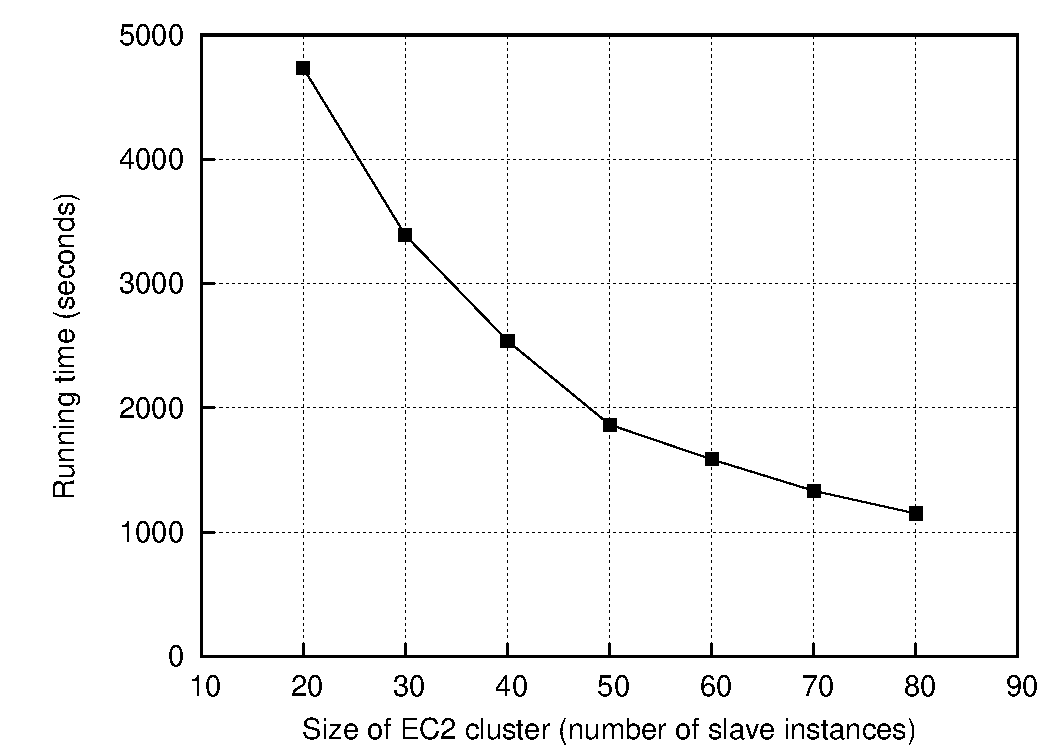
\includegraphics[scale=0.45]{figures/fig-ch3-pairs-vs-stripes-ec2a.pdf}
\includegraphics[scale=0.45]{figures/fig-ch3-pairs-vs-stripes-ec2b.pdf}
\end{center}
\caption{Running time of the stripes algorithm on the APW corpus with
  Hadoop clusters of different sizes from EC2 (left).  Scaling
  characteristics (relative speedup) in terms of increasing Hadoop
  cluster size (right).}
\label{figure:chapter3:pairs-vs-stripes-ec2}
\end{figure}

An additional series of experiments explored the scalability of the
stripes approach along another dimension:\ the size of the cluster.
These experiments were made possible by Amazon's EC2 service, which
allows users to rapidly provision clusters of varying sizes for
limited durations (for more information, refer back to our discussion
of utility computing in Section~\ref{chapter1:clouds}).  Virtualized
computational units in EC2 are called instances, and the user is
charged only for the instance-hours consumed.
Figure~\ref{figure:chapter3:pairs-vs-stripes-ec2} (left) shows the
running time of the stripes algorithm (on the same corpus, with same
setup as before), on varying cluster sizes, from 20 slave ``small''
instances all the way up to 80 slave ``small'' instances (along the
\emph{x}-axis).  Running times are shown with solid squares.
Figure~\ref{figure:chapter3:pairs-vs-stripes-ec2} (right) recasts the
same results to illustrate scaling characteristics.  The circles plot
the relative size and speedup of the EC2 experiments, with respect to
the 20-instance cluster.  These results show highly desirable linear
scaling characteristics (i.e., doubling the cluster size makes the job
twice as fast).  This is confirmed by a linear regression with an
$R^2$ value close to one.

Viewed abstractly, the pairs and stripes algorithms represent two
different approaches to counting co-occurring events from a large
number of observations.  This general description captures the gist of
many algorithms in fields as diverse as text processing, data mining,
and bioinformatics.  For this reason, these two design patterns are
broadly useful and frequently observed in a variety of applications.

To conclude, it is worth noting that the pairs and stripes approaches
represent endpoints along a continuum of possibilities.  The pairs
approach individually records \emph{each} co-occurring event, while the
stripes approach records \emph{all} co-occurring events with respect a
conditioning event.  A middle ground might be to record a subset of
the co-occurring events with respect to a conditioning event.  We
might divide up the entire vocabulary into $b$ buckets (e.g., via
hashing), so that words co-occurring with $w_i$ would be divided into
$b$ smaller ``sub-stripes'', associated with ten separate keys,
$(w_i,1), (w_i,2) \ldots (w_i,b)$.  This would be a reasonable
solution to the memory limitations of the stripes approach, since each
of the sub-stripes would be smaller.  In the case of $b=|V|$, where
$|V|$ is the vocabulary size, this is equivalent to the pairs
approach.  In the case of $b=1$, this is equivalent to the standard
stripes approach.

\section{Computing Relative Frequencies}
\label{chapter3:cond-prob}

Let us build on the pairs and stripes algorithms presented in the
previous section and continue with our running example of constructing
the word co-occurrence matrix $M$ for a large corpus.  Recall that in
this large square $n \times n$ matrix, where $n=|V|$ (the vocabulary
size), cell $m_{ij}$ contains the number of times word $w_i$ co-occurs
with word $w_j$ within a specific context.  The drawback of absolute
counts is that it doesn't take into account the fact that some words
appear more frequently than others.  Word $w_i$ may co-occur
frequently with $w_j$ simply because one of the words is very common.
A simple remedy is to convert absolute counts into relative
frequencies, $f(w_j|w_i)$.  That is, what proportion of the time does
$w_j$ appear in the context of $w_i$?  This can be computed using the
following equation:
\begin{align}
f(w_j|w_i) = \frac{N(w_i,w_j)}{\sum_{w'}{N(w_i,w')}}
\end{align}

\noindent Here, $N(\cdot, \cdot)$ indicates the number of times a
particular co-occurring word pair is observed in the corpus.  We need
the count of the joint event (word co-occurrence), divided by what is
known as the marginal (the sum of the counts of the conditioning
variable co-occurring with anything else).

Computing relative frequencies with the stripes approach is
straightforward.  In the reducer, counts of all words that co-occur
with the conditioning variable ($w_i$ in the above example) are
available in the associative array.  Therefore, it suffices to sum all
those counts to arrive at the marginal (i.e., $\sum_{w'}{N(w_i,w')}$),
and then divide all the joint counts by the marginal to arrive at the
relative frequency for all words.  This implementation requires
minimal modification to the original stripes algorithm in
Algorithm~\ref{algorithm:chapter3:coocur:stripes}, and illustrates the use
of complex data structures to coordinate distributed computations in
MapReduce.  Through appropriate structuring of keys and values, one
can use the MapReduce execution framework to bring together all the
pieces of data required to perform a computation.  Note that, as with
before, this algorithm also assumes that each associative array fits
into memory.

How might one compute relative frequencies with the pairs approach?
In the pairs approach, the reducer receives $(w_i, w_j)$ as the key and
the count as the value.  From this alone it is not possible to compute
$f(w_j|w_i)$ since we do not have the marginal.  Fortunately, as in the
mapper, the reducer can preserve state across multiple keys.  Inside
the reducer, we can buffer in memory all the words that co-occur with
$w_i$ and their counts, in essence building the associative array in the
stripes approach.  To make this work, we must define the sort order of
the pair so that keys are first sorted by the left word, and then by
the right word.  Given this ordering, we can easily detect if all
pairs associated with the word we are conditioning on ($w_i$) have been
encountered.  At that point we can go back through the in-memory
buffer, compute the relative frequencies, and then emit those results
in the final key-value pairs.

There is one more modification necessary to make this algorithm work.
We must ensure that all pairs with the same left word are sent to the
same reducer.  This, unfortunately, does not happen
automatically:\ recall that the default partitioner is based on the
hash value of the intermediate key, modulo the number of reducers.
For a complex key, the raw byte representation is used to compute the
hash value.  As a result, there is no guarantee that, for example,
(dog, aardvark) and (dog, zebra) are assigned to the same reducer.  To
produce the desired behavior, we must define a custom partitioner that
only pays attention to the left word.  That is, the partitioner should
partition based on the hash of the left word only.

This algorithm will indeed work, but it suffers from the same drawback
as the stripes approach:\ as the size of the corpus grows, so does
that vocabulary size, and at some point there will not be sufficient
memory to store all co-occurring words and their counts for the word
we are conditioning on.  For computing the co-occurrence matrix, the
advantage of the pairs approach is that it doesn't suffer from any
memory bottlenecks.  Is there a way to modify the basic pairs approach
so that this advantage is retained?

As it turns out, such an algorithm is indeed possible, although it
requires the coordination of several mechanisms in MapReduce.  The
insight lies in properly sequencing data presented to the reducer.  If
it were possible to somehow compute (or otherwise obtain access to)
the marginal in the reducer before processing the joint counts, the
reducer could simply divide the joint counts by the marginal to
compute the relative frequencies.  The notion of ``before'' and
``after'' can be captured in the ordering of key-value pairs, which
can be explicitly controlled by the programmer.  That is, the
programmer can define the sort order of keys so that data needed
earlier is presented to the reducer before data that is needed later.
However, we still need to compute the marginal counts.  Recall that in
the basic pairs algorithm, each mapper emits a key-value pair with the
co-occurring word pair as the key.  To compute relative frequencies,
we modify the mapper so that it additionally emits a ``special'' key
of the form $(w_i, \ast)$, with a value of one, that represents the
contribution of the word pair to the marginal.  Through use of
combiners, these partial marginal counts will be aggregated before
being sent to the reducers.  Alternatively, the in-mapper combining
pattern can be used to even more efficiently aggregate marginal
counts.

In the reducer, we must make sure that the special key-value pairs
representing the partial marginal contributions are processed before
the normal key-value pairs representing the joint counts.  This is
accomplished by defining the sort order of the keys so that pairs with
the special symbol of the form $(w_i, \ast)$ are ordered before any other
key-value pairs where the left word is $w_i$.  In addition, as with
before we must also properly define the partitioner to pay attention
to only the left word in each pair.  With the data properly sequenced,
the reducer can directly compute the relative frequencies.

\begin{figure}[t]
\begin{tabular}{lll}
\textbf{key} & \textbf{values} &  \\
$(\textrm{dog}, \ast)$        & $[$6327, 8514, $\ldots$$]$ & compute marginal: \\
 & & $\sum_{w'}{N(\textrm{dog},w')} = 42908$\\
$(\textrm{dog}, \textrm{aardvark})$ & $[$2,1$]$    & $f(\textrm{aardvark}|\textrm{dog}) = 3/42908$ \\
$(\textrm{dog}, \textrm{aardwolf})$ & $[$1$]$      & $f(\textrm{aardwolf}|\textrm{dog}) = 1/42908$ \\
\ldots            &      & \\
$(\textrm{dog}, \textrm{zebra})$    & $[$2,1,1,1$]$    & $f(\textrm{zebra}|\textrm{dog}) = 5/42908$ \\
$(\textrm{doge}, \ast)$       & $[$682, $\ldots$$]$  & compute marginal: \\
&& $\sum_{w'}{N(\textrm{doge},w')} = 1267$\\
\ldots            &      & \\
\end{tabular}
\caption{Example of the sequence of key-value pairs presented to the
  reducer in the pairs algorithm for computing relative frequencies.
  This illustrates the application of the order inversion design
  pattern.}
\label{figure:chapter3:cond-prob-reducer}
\end{figure}

A concrete example is shown in
Figure~\ref{figure:chapter3:cond-prob-reducer}, which lists the
sequence of key-value pairs that a reducer might encounter.  First,
the reducer is presented with the special key $(\textrm{dog}, \ast)$
and a number of values, each of which represents a partial marginal
contribution from the map phase (assume here either combiners or
in-mapper combining, so the values represent partially aggregated
counts).  The reducer accumulates these counts to arrive at the
marginal, $\sum_{w'}{N(\textrm{dog},w')}$.  The reducer holds on to
this value as it processes subsequent keys.  After $(\textrm{dog},
\ast)$, the reducer will encounter a series of keys representing joint
counts; let's say the first of these is the key $(\textrm{dog},
\textrm{aardvark})$.  Associated with this key will be a list of
values representing partial joint counts from the map phase (two
separate values in this case).  Summing these counts will yield the
final joint count, i.e., the number of times dog and aardvark co-occur
in the entire collection.  At this point, since the reducer already
knows the marginal, simple arithmetic suffices to compute the relative
frequency.  All subsequent joint counts are processed in exactly the
same manner.  When the reducer encounters the next special key-value
pair $(\textrm{doge}, \ast)$, the reducer resets its internal state
and starts to accumulate the marginal all over again.  Observe that
the memory requirement for this algorithm is minimal, since only the
marginal (an integer) needs to be stored.  No buffering of individual
co-occurring word counts is necessary, and therefore we have
eliminated the scalability bottleneck of the previous algorithm.

This design pattern, which we call ``order inversion'', occurs
surprisingly often and across applications in many domains.  It is so
named because through proper coordination, we can access the result of
a computation in the reducer (for example, an aggregate statistic)
before processing the data needed for that computation.  The key
insight is to convert the sequencing of computations into a sorting
problem.  In most cases, an algorithm requires data in some fixed
order:\ by controlling how keys are sorted and how the key space is
partitioned, we can present data to the reducer in the order necessary
to perform the proper computations.  This greatly cuts down on the
amount of partial results that the reducer needs to hold in memory.

To summarize, the specific application of the order inversion design
pattern for computing relative frequencies requires the
following:

\begin{itemize}

\item Emitting a special key-value pair for each co-occurring word
  pair in the mapper to capture its contribution to the marginal.

\item Controlling the sort order of the intermediate key so that the
  key-value pairs representing the marginal contributions are
  processed by the reducer before any of the pairs representing the
  joint word co-occurrence counts.

\item Defining a custom partitioner to ensure that all pairs with the
  same left word are shuffled to the same reducer.

\item Preserving state across multiple keys in the reducer to first
  compute the marginal based on the special key-value pairs and then
  dividing the joint counts by the marginals to arrive at the
  relative frequencies.

\end{itemize}

\noindent As we will see in Chapter~\ref{chapter-indexing}, this design
pattern is also used in inverted index construction to properly set
compression parameters for postings lists.

\section{Secondary Sorting}
\label{chapter3:secondary-sorting}

MapReduce sorts intermediate key-value pairs by the keys during the
shuffle and sort phase, which is very convenient if computations
inside the reducer rely on sort order (e.g., the order inversion
design pattern described in the previous section).  However, what if
in addition to sorting by key, we also need to sort by value?
Google's MapReduce implementation provides built-in functionality for
(optional) secondary sorting, which guarantees that values arrive in
sorted order.  Hadoop, unfortunately, does not have this capability
built in.

Consider the example of sensor data from a scientific
experiment:\ there are $m$ sensors each taking readings on continuous
basis, where $m$ is potentially a large number.  A dump of the sensor
data might look something like the following, where $r_x$ after
each timestamp represents the actual sensor readings (unimportant for
this discussion, but may be a series of values, one or more complex
records, or even raw bytes of images).

\begin{quote}
$(t_1, m_1, r_{80521})$\\
$(t_1, m_2, r_{14209})$\\
$(t_1, m_3, r_{76042})$\\
$...$\\
$(t_2, m_1, r_{21823})$\\
$(t_2, m_2, r_{66508})$\\
$(t_2, m_3, r_{98347})$
\end{quote}

\noindent Suppose we wish to reconstruct the activity at each
individual sensor over time.  A MapReduce program to accomplish this
might map over the raw data and emit the sensor id as the intermediate
key, with the rest of each record as the value:

\begin{quote}
$m_1 \rightarrow (t_1, r_{80521})$
\end{quote}

\noindent This would bring all readings from the same sensor together
in the reducer.  However, since MapReduce makes no guarantees about
the ordering of values associated with the same key, the sensor
readings will not likely be in temporal order.  The most obvious
solution is to buffer all the readings in memory and then sort by
timestamp before additional processing.  However, it should be
apparent by now that any in-memory buffering of data introduces a
potential scalability bottleneck.  What if we are working with a high
frequency sensor or sensor readings over a long period of time?  What
if the sensor readings themselves are large complex objects?  This
approach may not scale in these cases---the reducer would run out of
memory trying to buffer all values associated with the same key.

This is a common problem, since in many applications we wish to first
group together data one way (e.g., by sensor id), and then sort within
the groupings another way (e.g., by time).  Fortunately, there is a
general purpose solution, which we call the ``value-to-key
conversion'' design pattern.  The basic idea is to move part of the
value into the intermediate key to form a composite key, and let the
MapReduce execution framework handle the sorting.  In the above
example, instead of emitting the sensor id as the key, we would emit
the sensor id and the timestamp as a composite key:

\begin{quote}
$(m_1, t_1) \rightarrow (r_{80521})$
\end{quote}

\noindent The sensor reading itself now occupies the value.  We must
define the intermediate key sort order to first sort by the sensor id
(the left element in the pair) and then by the timestamp (the right
element in the pair).  We must also implement a custom partitioner so
that all pairs associated with the same sensor are shuffled to the
same reducer.

Properly orchestrated, the key-value pairs will be presented to the
reducer in the correct sorted order:

\begin{quote}
$(m_1, t_1) \rightarrow [(r_{80521})]$ \\
$(m_1, t_2) \rightarrow [(r_{21823})]$ \\
$(m_1, t_3) \rightarrow [(r_{146925})]$ \\
$\ldots$
\end{quote}

\noindent However, note that sensor readings are now split across
multiple keys.  The reducer will need to preserve state and keep track
of when readings associated with the current sensor end and the next
sensor begin.\footnote{Alternatively, Hadoop provides API hooks to
  define ``groups'' of intermediate keys that should be processed
  together in the reducer.}

The basic tradeoff between the two approaches discussed above (buffer
and in-memory sort vs.\ value-to-key conversion) is where sorting is
performed.  One can explicitly implement secondary sorting in the
reducer, which is likely to be faster but suffers from a scalability
bottleneck.\footnote{Note that, in principle, this need not be an
  in-memory sort.  It is entirely possible to implement a disk-based
  sort within the reducer, although one would be duplicating
  functionality that is already present in the MapReduce execution
  framework.  It makes more sense to take advantage of functionality
  that is already present with value-to-key conversion.}  With
value-to-key conversion, sorting is offloaded to the MapReduce
execution framework.  Note that this approach can be arbitrarily
extended to tertiary, quaternary, etc.\ sorting.  This pattern results
in many more keys for the framework to sort, but distributed sorting
is a task that the MapReduce runtime excels at since it lies at the
heart of the programming model.

\section{Summary}

This chapter provides a guide on the design of MapReduce algorithms.
In particular, we present a number of ``design patterns'' that capture
effective solutions to common problems.  In summary, they are:

\begin{itemize}

\item ``In-mapper combining'', where the functionality of the combiner
  is moved into the mapper.  Instead of emitting intermediate output
  for every input key-value pair, the mapper aggregates partial
  results across multiple input records and only emits intermediate
  key-value pairs after some amount of local aggregation is performed.

\item The related patterns ``pairs'' and ``stripes'' for keeping track
  of joint events from a large number of observations.  In the pairs
  approach, we keep track of each joint event separately, whereas in
  the stripes approach we keep track of all events that co-occur with
  the same event.  Although the stripes approach is significantly more
  efficient, it requires memory on the order of the size of the event
  space, which presents a scalability bottleneck.

\item ``Order inversion'', where the main idea is to convert the
  sequencing of computations into a sorting problem.  Through careful
  orchestration, we can send the reducer the result of a computation
  (e.g., an aggregate statistic) before it encounters the data
  necessary to produce that computation.

\item ``Value-to-key conversion'', which provides a scalable solution
  for secondary sorting.  By moving part of the value into the key, we
  can exploit the MapReduce execution framework itself for sorting.

\end{itemize}

\noindent Ultimately, controlling synchronization in the MapReduce
programming model boils down to effective use of the following
techniques:

\begin{enumerate}

\item Constructing complex keys and values that bring together data
  necessary for a computation.  This is used in all of the above
  design patterns.

\item Executing user-specified initialization and termination code in
  either the mapper or reducer.  For example, in-mapper combining
  depends on emission of intermediate key-value pairs in the map task
  termination code.

\item Preserving state across multiple inputs in the mapper and
  reducer.  This is used in in-mapper combining, order inversion, and
  value-to-key conversion.

\item Controlling the sort order of intermediate keys.  This is used
  in order inversion and value-to-key conversion.

\item Controlling the partitioning of the intermediate key space.
  This is used in order inversion and value-to-key conversion.

\end{enumerate}

\noindent This concludes our overview of MapReduce algorithm design.
It should be clear by now that although the programming model forces
one to express algorithms in terms of a small set of rigidly-defined
components, there are many tools at one's disposal to shape the flow
of computation.  In the next few chapters, we will focus on specific
classes of MapReduce algorithms:\ for inverted indexing in
Chapter~\ref{chapter-indexing}, for graph processing in
Chapter~\ref{chapter-graphs}, and for expectation-maximization in
Chapter~\ref{chapter6}.
